\documentclass[a4paper,14pt]{article}
\usepackage{extsizes}
\usepackage[T2A]{fontenc}
\usepackage[utf8x]{inputenc}
\usepackage[english,russian]{babel}
\usepackage{amssymb,amsfonts,amsmath,mathtext,cite,enumerate,float}
% \usepackage[dvips]{graphicx}
%\usepackage{breqn}
\usepackage{graphicx}
\usepackage{sectsty}
\usepackage{array}
\usepackage{amsthm}
\usepackage{titlesec}
\usepackage{indentfirst}
\usepackage{xr}
\usepackage{subfigure}
\usepackage[round, sort, numbers]{natbib}
\usepackage{url}
\usepackage{setspace}
\usepackage{pdfpages}
\usepackage{caption}

\setcitestyle{square}
\graphicspath{{images/}}

\allsectionsfont{\centering}

\makeatletter
% \renewcommand{\@biblabel}[1]{#1.}
\makeatother

\usepackage{geometry}
\geometry{left=2.5cm}
\geometry{right=1.5cm}
\geometry{top=2cm}
\geometry{bottom=2cm}

\newcommand{\norm}[1]{\left\lVert#1\right\rVert}
\newcommand{\isum}[2][j]{\sum \limits_{#1=1}^{\infty}{#2}}
\newcommand{\operator}[1]{\mathcal{R}{#1}}
\newcommand{\supp}{\mathop{\mathrm{supp}}}
\newtheorem{remark}{Замечание}

\DeclareMathOperator\arctanh{arctanh}
\DeclareMathOperator\arccoth{arccoth}
\DeclareMathOperator\arccot{arccot}

\numberwithin{equation}{section}

\newcommand{\sectionbreak}{\clearpage}

\begin{document}

%\includepdf[pages={1}]{titul.pdf}
\renewcommand{\contentsname}{Содержание}
\tableofcontents

\onehalfspacing
\begin{onehalfspace}
    \section*{Введение}
\addcontentsline{toc}{section}{Введение}
\vspace{1em}

В реальных физических процессах неизбежно возникают непредусмотренные 
флуктуации, и поэтому возникает необходимость разработки методов построения 
управлений, способных реагировать на непредусмотренные возмущения и подавлять 
их \cite{Furs}. Проблемы стабилизации систем параболического типа привлекают внимание 
специалистов в силу прикладной значимости данной системы \cite{Chebotarev}. 
Управления такого типа называются \emph{управлениями с обратной связью} \cite{KS}.

Вопрос о стабилизируемости различных эволюционных уравнений в частных 
производных с помощью управлений исследовался многими авторами, среди которых 
A.Kwiecinka \cite{KWCK}, Barbu V. \cite{Barbu}, M. Kristic
\cite{KMV, KS}, Фурсиков А.В. \cite{Furs}, Чеботарёв А.Ю. 
\cite{Chebotarev, ChebotarevBS, ChebotarevMGT} и разработаны методы управления, 
такие как : стабилизация Ляпунова, метод backstepping, управление с обратной связью.

В представленной ВКР рассматривается стабилизация эволюционных систем с 
постоянными коэффициентами конечномерным локальным управлением с обратной связью.

    \section{Стабилизация неустойчивых параболических систем}
\vspace{1em}

\subsection{Анализ устойчивости линейного параболического уравнения}

Рассмотрим параболическое уравнение

\begin{equation}\label{dif_form}
    u_t = u_{xx} + \alpha u, \ x \in \Omega, \ t > 0
\end{equation}
с начальным и граничными условиями:
\begin{gather}\label{d_control}
    u(0, t) = u(1, t) = 0, \\*
    u(x, 0) = u_{0}(x) \in H. \nonumber
\end{gather}

Умножим уравнение \eqref{dif_form} на $u$ скалярно в $H$

\begin{equation*}
    (u_t, u) = (u_{xx}, u) + \alpha (u, u).
\end{equation*}

Скалярное произведение в $H$ определяется как $(u, v) = \int_0^1 uv dx$,
а норма как $\norm{u} = \sqrt{(u, u)}$. Получаем

\begin{equation}\label{int_form}
    \frac{1}{2}\frac{d}{dt}\norm{u}^2 = -\norm{u_x}^2 + \alpha \norm{u}^2.
\end{equation}
C помощью неравенства Пуанкаре–Фридрихса-Стеклова
\begin{equation*}
    \norm{u}^2 \le \frac{1}{\pi^2} \norm{u_x}^2
\end{equation*}
получаем следующую оценку 
\begin{equation}\label{stable_opr}
    \frac{1}{2}\frac{d}{dt}\norm{u}^2 \le (\alpha - \pi^2)\norm{u}^2.
\end{equation}
Рассмотрим 3 случая.

\begin{enumerate}
    \item $\alpha = \pi^2$. Тогда из \eqref{stable_opr} следует неравенство
        \begin{equation}
            \norm{u}^2 \le \norm{u_0}^2.
        \end{equation}

        Указанное неравенство означает, что нулевое решение задачи
        \eqref{dif_form} - \eqref{d_control} устойчиво по Ляпунову, но не 
        устойчиво ассимптотически.

    \item $\alpha < \pi^2$. Обозначим $\frac{\mu}{2} = -(\alpha - \pi^2)$,\\

        тогда

        \begin{equation}\label{less_pi2}
            \frac{d}{dt}\norm{u}^2 + \mu \norm{u}^2 \le 0.
        \end{equation}

        Домножим обе части \eqref{less_pi2} на $e^{\mu t}$. Тогда, 
        $\frac{d(\norm{u}^2 e^{\mu t})}{dt} \le 0$. Проинтегрируем по $t$ и в 
        итоге получим

        \begin{equation*}
            \norm{u}^2 \le \norm{u_0}^2 e^{-\mu t} = \norm{u_0}^2 e^{2(\alpha -
            \pi^2) t}.
        \end{equation*}

        Данная оценка гарантирует ассимптитическую экспоненциальную устойчивость.

    \item $\alpha > \pi^2$. Решение начально краевой задачи 
        \eqref{dif_form} - \eqref{d_control} имеет вид
        \begin{equation}
            u(x, t) = 2 \isum{a_j e^{(\alpha - \pi^2 j^2)t}\sin{(\pi j x)}},
        \end{equation}

        здесь $a_j = \int_0^1{u_0 \sin{(\pi j s)} ds}$. Первый член суммы 
        $a_1e^{(\alpha - \pi^2j^2)t}\sin(\pi j x)$ указывает на темп роста 
        решения при $t \rightarrow \infty$. Следовательно, система неустойчива.
\end{enumerate}

Для стабилизации системы \eqref{int_form} в случае 3, будем использовать ниже 
описанный метод, предложенный Чеботаревым А.Ю. \cite{ChebotarevMGT}

    \subsection{Примеры неустойчивых решений уравнения теплопроводности}
\vspace{1em}

\newtheorem{exmp}{Пример}

\begin{exmp}
\end{exmp}

В качестве начальных условий возмем $u_0 = sin(\pi x)$. Продемонстрируем 
неустойчивость нулевого решения при $\alpha = \pi^2 + 0.1$.

\begin{figure}[H]
    \centering
        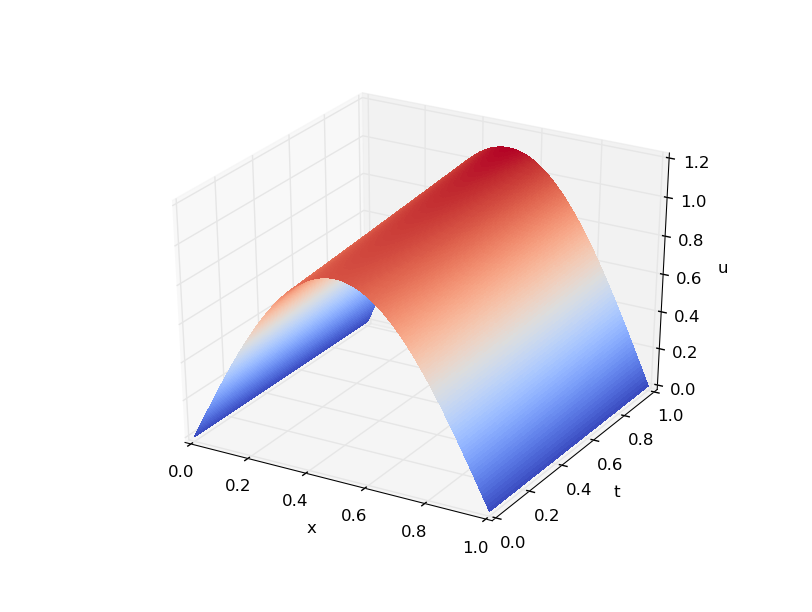
\includegraphics[width=3.5in]{par_ex_pi01}
        \caption{Без управления}
        \label{fig:test1}
\end{figure}

\begin{exmp}
\end{exmp}

Пусть $u(x, 0) = x(1 - x)$ - начальное условие . Заведомо выберем параметр 
$\alpha = \pi^2 + 3$ большим. 

\begin{figure}[H]
    \centering
        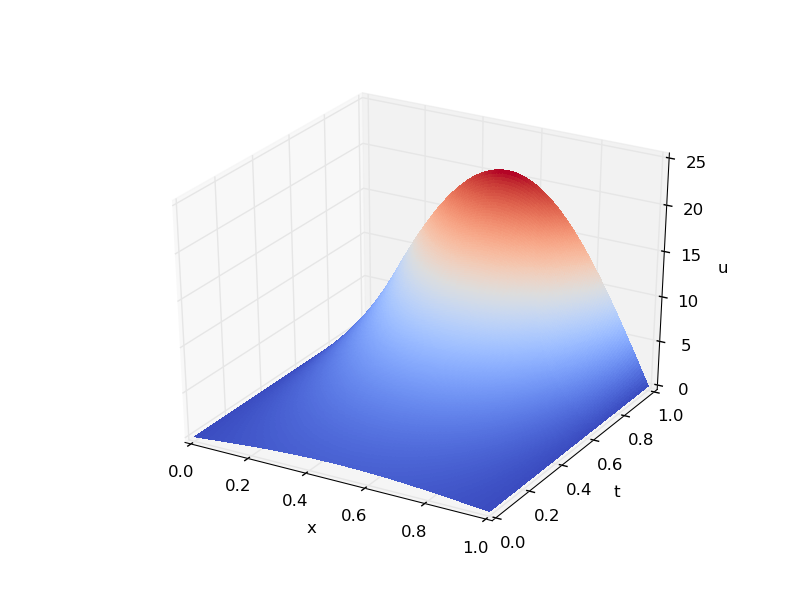
\includegraphics[width=3.5in]{par_ex_pi3}
        \caption{Без управления}
        \label{fig:test1}
\end{figure}


    \subsection{Стабилизация конечномерным локальным управлением с обратной связью}
\vspace{1em}

Рассмотрим систему

\begin{equation}\label{ndif_form}
    u_t = u_{xx} + \alpha u, \ 0 < x < 1, \ t > 0.
\end{equation}
с начальным и граничными условиями
\begin{gather}
    u(0, t) = u(1, t) = 0, \\*
    u(x, 0) = u_{0}(x) \in H .\nonumber
\end{gather}
Здесь и далее $H = L^2(\Omega)$.\\

Как показано в \S 1, в случае, когда $\alpha > \pi^2$, нулевое решение уравнения 
\eqref{ndif_form} неустойчиво.
Задача стабилизации параболического уравнения, заданного в ограниченной области,
заключается в построении такого оператора управления, чтобы решение смешанной 
краевой задачи стремилось (при $t \rightarrow \infty$) к заданному стационарному 
решению с предписанной скоростью $e^{(-\delta_0t)}$.

Сформулируем задачу стабилизации неустойчивого нулевого решения уравнения 
\eqref{ndif_form} за счет локального управления.\\

Пусть $\omega \subset (0, 1)$ - произвольный интеравал такой, что 
$\bar{\omega} \subset (0, 1)$.Задача стабилизации за счет конечномерных локально 
распределённых в $\omega$ управлений заключается в построении оператора 
$\mathcal{R} : H \rightarrow H$ такого, что

\begin{enumerate}
    \item $\forall z \in H \ \mathbf{supp} \ \operator{z} \subset \omega$,
    \item $\dim \operator{(H)} < +\infty$.
\end{enumerate}
и при этом решение задачи
\begin{gather}
    u_t - u_{xx} - \alpha u = \operator{u}. \nonumber\\
    u(0, t) = u(1, t) = 0, \ u(x, 0) = u_0. \nonumber
\end{gather}
экспоненциально стремится к нулю при $t \rightarrow + \infty$.

\subsection{Конструкция оператора управления}
\vspace{1em}

Заметим, что функции

\begin{equation}\label{basis}
    w_j = w_j(x) = \sqrt{2}\sin{(\pi j x)}, \ x \in (0, 1), \ j=1, 2, ..
\end{equation}
образуют базис в $H$ и в $V$, причем в $H$ базиc ортонормирован.\\
Через $H_m$ обозначим подпространство в $H$, образованное первыми $m$ функциями 
из \eqref{basis}.\\

Далее рассмотрим следующие операторы проектирования

$$P_m : H \rightarrow H_m, \ Q_m : H \rightarrow H_m^{\perp}.$$

\begin{equation}
    P_m u = \sum \limits_{j=1}^{m} {(u, w_j) w_j}.
\end{equation}

\begin{equation}
    Q_m u = (I - P_m)u(x) = \sum \limits_{j=m + 1}^{\infty} {(u, w_j) w_j}.
\end{equation}

В качестве оператора стабилизиции будем рассматривать следующий конечномерный
оператор

$$\operator{z} = -r\chi_{\omega}P_mz, \ r > 0,$$
здесь
\begin{gather*}
    \begin{matrix}
        \chi_{\omega}(x) & =
        & \left\{
        \begin{matrix}
            0, & \mbox{если } x \notin \omega, \\
            1, & \mbox{иначе. }
        \end{matrix} \right.
    \end{matrix}
\end{gather*}

В следующем параграфе будет доказано, что существуют подходящие параметры 
$m \in \mathbb{N}$, $r = r_m > 0$, при которых $\operator{}$ обеспечивает 
стабилизацию неустойчивого решения.

\subsection{Теоретическое обоснование стабилизации}
\vspace{1em}

Рассмотрим уравнение
\begin{gather}\label{control}
    u_t - u_{xx} - \alpha u = -r\chi_{\omega}\varphi,\\*
    u|_{x = 0;1} = 0.
\end{gather}
Здесь $\varphi = P_mu$. Домножим скалярно обе части \eqref{control} на
$\varphi$. Учтем, что

\begin{gather*}
    (u, \varphi) = \norm{\varphi}^2,\\*
    (u_t, \varphi) = (\varphi_t, \varphi) = \frac{1}{2} \frac{d}{dt}
    \norm{\varphi}^2, \\*
    (u_{xx}, \varphi) = (\varphi_{xx}, \varphi) = -(\varphi_x, \varphi_x) = -
    \norm{\varphi_x}^2, \\*
    (\chi_{\omega}\varphi, \varphi) = \norm{\varphi}^2_{\omega}.
\end{gather*}
Тогда
\begin{equation*}
    \frac{1}{2} \frac{d}{dt} \norm{\varphi}^2  + \norm{\varphi_x}^2 - 
    \alpha \norm{\varphi}^2 + r \norm{\varphi}^2_{\omega} = 0.
\end{equation*}
Воспользуемся неравенством Пуанкаре-Фридрихса-Стеклова

\begin{equation}
    \norm{\varphi}^2 \le \frac{1}{\pi^2} \norm{\varphi_x}^2.
\end{equation}
В итоге получаем

\begin{equation}
    \frac{1}{2} \frac{d}{dt} \norm{\varphi}^2 + \pi^2 \norm{\varphi}^2 - 
    \alpha \norm{\varphi}^2 + r \norm{\varphi}^2_{\omega} \le 0.
\end{equation}

Приведём полезные для доказательства стабилизируемости леммы.

\newtheorem{lemma}{Лемма}

\begin{lemma}\label{util_lemma}
    Система $\left\{ w_j|_{\omega} \right\}^m_1$ линейно независима.
\end{lemma}

\begin{proof}
    % Пусть $D$ - оператор дифференцирования. Он является линейным отображением(преобразованием) $\mathbb{R}^m$ в $\mathbb{R}^m$. Рассмотрим следующее равенство :\\
    Cистема $\left\{ w_j|_{\omega} \right\}^m_1$ линейно независима, если 
    тождество ввида
    
    \begin{equation}\label{sum_func}
        \sum \limits_{j = 1}^m{c_j w_j(x)} = 0, \ x \in \omega.
    \end{equation}
    выполняется только при $c_1 = c_2 = ... = c_m = 0.$\\

    Пусть $D$ оператор дифференцирования, действующий в пространстве бесконечно 
    дифференцируемых функций.
    Заметим, что $D^2 w_j = -(\pi k)^2 w_j$. Подействуем  на \eqref{sum_func} 
    оператором $D^{2l}$ раз

    \begin{equation*}
        c_m (\pi m)^{2l} w_m + \sum \limits_{j = 1}^{m - 1}{c_j (\pi j)^{2l}
        w_j(x)} = 0.
    \end{equation*}

    Разделим на $(\pi m)^{2l}$. Тогда

    \begin{equation*}
        c_m w_m + \sum \limits_{j = 1}^{m - 1}{c_j \left(\frac{j}{m}\right)^{2l}
        w_j(x)}.
    \end{equation*}
    Заметим, что при $l \rightarrow +\infty$, правое слагаемое стремится к 0.\\
    Следовательно,

    \begin{equation*}
        c_m w_m = 0.
    \end{equation*}

    Функция $w_m(x) = \sin{(\pi m x)}$ не может принимать нулевые значения на 
    целом интервале, следовательно $c_m = 0$. Проделав те же самые рассуждения 
    для $\sum \limits_{j = 1}^{m - 1}{c_j w_j(x)}$, получаем что

    \begin{equation*}
        c_1 = c_2 = ... = c_m = 0.
    \end{equation*}

\end{proof}

\par
\vspace{2ex}

\begin{lemma}\label{main_lemma}
    \begin{equation}
        \gamma = \inf{ \left\{ \norm{z}^2_{\omega} : z = P_mu,\enskip u \in H, 
        \enskip \norm{z} = 1 \ \right\} } > 0.
    \end{equation}
    Здесь $\norm{z}^2_{\omega} = \int\limits_{\omega}{z^2dx}$.
\end{lemma}

\begin{proof}

    Рассмотрим функцию $f$, определённую на единичной сфере в $\mathbb{R}^m$

    \begin{equation}
       f(c_1, c_2, ..., c_m) = \int \limits_{\omega} {(\sum\limits_1^m {c_jw_j})^2}
       \text{, где } c_1^2 + c_2^2 + ... + c^2_m = 1.
    \end{equation}
    По теореме Вейштрасса, существует функция 
    $z_0 = \sum\limits_1^m {c_j^0 w_j} \in H_m$, такая, что

    \begin{equation}
       \gamma = f(c_1^0, c_2^0, ..., c_m^0) = \inf \limits_{c_1^2 + .. + c_m^2 =
       1} {f}.
    \end{equation}

    Заметим, что из линейной независимости 
    $\left\{ \omega_j \right\}^m_1$(по лемме \ref{util_lemma}) следует 
    положительность $\gamma$.

\end{proof}

\par
\vspace{2ex}

Выберем число $m \in \mathbb{N}$ так, что

\begin{equation}
    q = [(\pi(m + 1))^2 - \alpha - 1] > 0.
\end{equation}
На основании леммы \ref{main_lemma} справедлива следующая оценка
\begin{equation*}
    \frac{1}{2} \frac{d}{dt} \norm{\varphi}^2 + (\pi^2 - \alpha + r\gamma) 
    \norm{\varphi}^2 \le 0.
\end{equation*}

Далее, выберем число $r = r_m > 0$ так, чтобы
$\beta = \pi^2 - \alpha + r\gamma > 0$.
Умножим обе части неравенства на $2e^{2\beta t}$, интегрируем по $t$ и 
получаем следующую важную оценку

\begin{equation}\label{phi_mark}
    \norm{\varphi}^2 \le \norm{\varphi_0}^2 e^{-2\beta t},
\end{equation}
здесь $\varphi_0 = P_m u_0$
\vspace{2em}

Проведём аналогичные выкладки с $\psi = Q_m u$. Домножим обе части 
\eqref{control} скалярно на $\psi$. Учтем, что

\begin{gather*}
    (u, \psi) = \norm{\psi}^2,\\*
    (u_t, \psi) = (\psi_t, \psi) = \frac{1}{2} \frac{d}{dt} \norm{\psi}^2,\\*
    (u_{xx}, \psi) = (\psi_{xx}, \psi) = -(\psi_x, \psi_x) = -
    \norm{\psi_x}^2,\\*
    (\chi_{\omega}\varphi, \psi) = \int_{\omega}{\varphi \psi} \le
    \norm{\varphi} \norm{\psi}.
\end{gather*}
С помощью неравенства Пуанкаре-Фридрихса-Стеклова получаем оценку
\begin{equation}
    \norm{\psi}^2 \le (\frac{1}{\pi(m + 1)})^2 \norm{\psi_x}^2.
\end{equation}

Тогда

\begin{equation}\label{v2}
    \frac{1}{2} \frac{d}{dt} \norm{\psi}^2 + (\pi(m + 1))^2 \norm{\psi}^2 - 
    \alpha \norm{\psi}^2 \le r \norm{\varphi} \norm{\psi}.
\end{equation}

Рассмотрим подробнее \eqref{v2}.\\
Для оценки произведения норм, воспользуемся неравенством Юнга

\begin{equation*}
    \norm{\varphi} \norm{\psi} \le (\frac{\varepsilon \norm{\psi}^2}{2} + 
    \frac{\norm{\varphi}^2}{2 \varepsilon}),
\end{equation*}
здесь $\varepsilon = \frac{2}{r}$. Из \eqref{v2} получаем неравенства

\begin{equation*}
    \frac{1}{2} \frac{d}{dt} \norm{\psi}^2 + (\pi(m + 1))^2 \norm{\psi}^2 - 
    \alpha \norm{\psi}^2 \le r (\frac{\varepsilon \norm{\psi}^2}{2} + 
    \frac{\norm{\varphi}^2}{2 \varepsilon}).
\end{equation*}
\begin{equation*}
    \frac{1}{2} \frac{d}{dt} \norm{\psi}^2  + [(\pi(m + 1))^2 - \alpha - 1] 
    \norm{\psi}^2 \le \frac{r^2}{4}\norm{\varphi}^2 \le 
    \frac{r^2}{4}\norm{\varphi_0}^2 e^{-2\beta t}.
\end{equation*}
\begin{equation}
    \frac{1}{2} \frac{d}{dt} \norm{\psi}^2 + q\norm{\psi}^2 \le 
    \frac{r^2}{4}\norm{\varphi_0}^2 e^{-2\beta t}.
\end{equation}

Напомним, что $q > 0$ за счет выбора числа гармоник в операторе $P_m$.
Домножим обе части неравенства на $2e^{2qt}$ и проинтегрируем
\begin{gather*}
    \int\limits_0^t{d(e^{2q\tau}} \norm{\psi}^2) \le 
    \frac{r^2}{2} \norm{\varphi_0}^2 \frac{1}{2q - 2\beta} 
    \int\limits_0^t {e^{(2q -2\beta) \tau} d[(2q -2\beta) \tau]}\\*
    e^{2qt} \norm{\psi}^2 - \norm{\psi_0}^2 \le \frac{r^2}{2}
    \norm{\varphi_0}^2 \frac{1}{2q - 2\beta} e^{(2q -2\beta)t}.
\end{gather*}

Следовательно

\begin{equation}\label{psi_mark}
    \norm{\psi}^2 \le \norm{\psi_0}^2 e^{-2qt} + \frac{r^2}{2} 
    \norm{\varphi_0}^2 \frac{1}{2(q - \beta)} e^{-2\beta t}.
\end{equation}

Известно, что $u = \varphi + \psi$. Воспользуемся оценками норм $\psi$ и 
$\varphi$ [\eqref{psi_mark}, \eqref{phi_mark}] и получим

\begin{gather*}
    \norm{u}^2 = \norm{\varphi}^2 + \norm{\psi}^2 \le \norm{\varphi_0}^2 
    e^{-2\beta t} + \norm{\psi_0}^2 e^{-2qt} + \frac{r^2}{2} \norm{\varphi_0}^2 
    \frac{1}{2(q - \beta)} e^{-2\beta t}
\end{gather*}

Окончально, оценку стабилизации можно записать в виде

\begin{equation}
    \norm{u}^2 \le \norm{u_0}^2 \left( e^{-2\beta t} + e^{-2qt} + 
    \frac{r^2 e^{-2\beta t}}{4(q - \beta)} \right)
\end{equation}

    \subsection{Численная реализация алгоритма}
\vspace{1em}

В настоящем параграфе приведена численная реализация предложенного алгоритма 
стабилизации.\\

Рассмотрим задачу с стабилизирующим оператором

\begin{equation}\label{sys}
    u_t - u_{xx} - \alpha u = -r\chi_{\omega}P_m u, \ 0 < x < 1, \quad t > 0
\end{equation}

К уравнению \eqref{sys} добавим начальное и граничные условия

\begin{gather}\label{s_control}
    u(0, t) = u(1, t) = 0, \\*
    u(x, 0) = u_{0}(x) \in H. \nonumber
\end{gather}

Для \eqref{sys} запишем разностную схему

\begin{equation}\label{scheme}
    \frac{u^{j + 1}_i - u^j_i}{\tau} - \frac{u_{i + 1}^{j + 1} - 
    2u_{i}^{j + 1} + u_{i - 1}^{j + 1}}{h^2} - \alpha u_{i}^{j + 1} + 
    r\chi_{\omega}P_m u^j_i = 0.
\end{equation}

Запишем аппроксимацию начального и граничных условий

\begin{gather}
    u_i^0 = u_0(x_i), \\*
    u_1^{j+1} = u_N^{j+1} = 0. \nonumber
\end{gather}

Вспомним, что оператор проектирования имеет вид

\begin{gather*}
    P_m u = \sum \limits_{j=1}^{m} {(u, w_j) w_j} = 
    \sqrt{2} (\sum \limits_{j=1}^{m} {C_k \sin{(\pi k x)}}), \ \text{где }
    C_k = \sqrt{2} \int\limits_0^1{u(s)\sin{(\pi k s)} ds}.
\end{gather*}

Заметим, что $C_k$ - это интеграл от быстро осциллирующей функции вида

\begin{equation}
    \int\limits_a^b{f(x) e^{i\omega x} dx} \approx \int\limits_a^b{L_3(x)
    e^{i\omega x} dx}.
\end{equation}

Поскольку, функция $f$ является гладкой, то на $[a, b]$ она легко приближается 
с известной погрешностью интерполяционными многочленами. Пусть для 
определенности, это интерполяционный многочлен в форме Лагранжа

\begin{equation}
    L_3(x) = P_1(x)f(x_1) + P_2(x)f(x_2) + P_3(x)f(x_3)
\end{equation}
построенный по узлам $x_1 = a$, $x_2 = \frac{a + b}{2}$, $x_3 = b$. $P_i$ - 
многочлены второй степени, не зависящие от функции $f$. Данный метод 
приближенного интегрирования называется формулой Филона. Именно этим 
способом и будем аппроксимировать оператор $P_m$.\\

Для решения данной схемы \eqref{scheme} воспользуемся методом прогонки.

    \subsection{Примеры численного моделирования стабилизации}

\vspace{1em}

\newtheorem{exmp_st}{Пример}

\begin{exmp_st}
\end{exmp_st}

В качестве начальных условий возмем $u_0 = \sin(\pi x)$. Продемонстрируем 
стабилизацию системы при $\alpha = \pi^2 + 0.1$. Фиксируем $\omega = [0, 0.2]$. 
Необходимо подобрать параметры $m$, $r_m$ так, чтобы $\beta > 0$ и $q > 0$. 
Рассмотрим подробнее $q = [(\pi(m + 1))^2 - \alpha - 1]$. При заданном 
$\alpha = \pi^2 + 0.1$, достаточно взять $m = 2$ для выполнения неравенства. 
Параметр $r$ придется подобрать так, чтобы решение стремилось к нулю.


\begin{figure}[H]
    \centering
    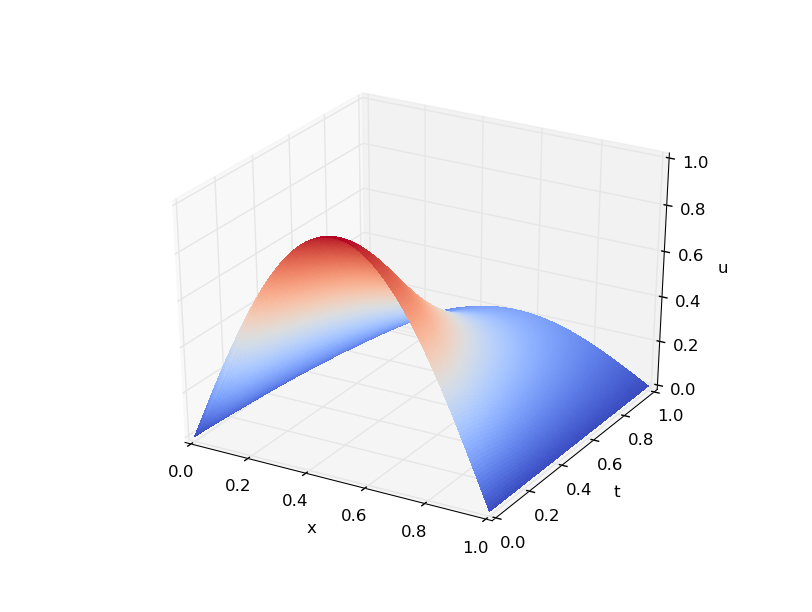
\includegraphics[width=4in]{par_re_pi01}
    \caption{Управление $m = 2,\; r = 8$}
    \label{fig:test2}
\end{figure}

\begin{exmp_st}
\end{exmp_st}

Пусть $u(x, 0) = x(1 - x)$ - начальное условие . Заведомо выберем параметр 
$\alpha = \pi^2 + 3$ большим. Зафиксируем $\omega = (0, 0.4)$. 
Необходимо подобрать $m$, таким чтобы $q > 0$. При $m \ge 2$ условие выполняется, 
поэтому мы фиксируем $m = 2$. На рис.4 показано, как быстро растет решение 
задачи \eqref{sys} - \eqref{s_control} при небольшом увеличении $\alpha$. 
Стабилизация этой системы представлена на рисунке 5

\begin{figure}[H]
    \centering
    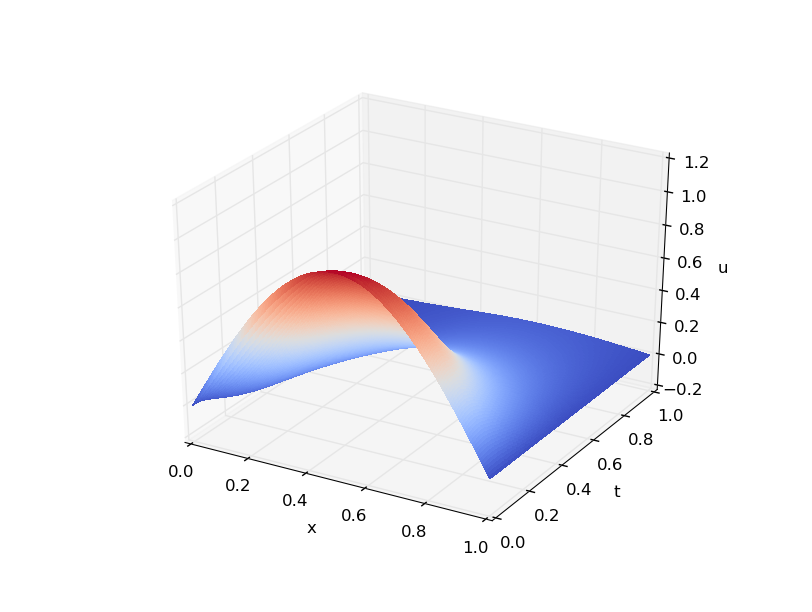
\includegraphics[width=4in]{par_re_pi3}
    \caption{Управление $m = 2,\; r = 15$}
    \label{fig:test2}
\end{figure}

    \section{Стабилизация неустойчивых стационарных решений уравнения Бюргерса}
\vspace{1em}

\subsection{Постановка задачи}

Рассмотрим уравнение Бюргерса с вязкостью $\nu > 0$ на интервале $\Omega = (0,
1) \subset \mathbb{R}$

\begin{equation}\label{burger}
    u_t - \nu u_{xx} + u_x u = f + y, \ u|_{\Gamma} = u_b, \quad t > 0
\end{equation}

Функция $f = f(x)$, $x \in \Omega$ является заданной, а функция $y = y(x, u)$
рассматривается как управление, носитель которого при фиксированном $t > 0$
содержиться в $\bar{\omega}$, где $\bar{\omega}$ - заданная подобласть $\Omega$.
Через $\Gamma = \{0, 1\}$ обозначена граница $\Omega$, $u_b \in \mathbb{R}^2$\\

Пусть $U$ - стационарное решение \eqref{burger}, то есть

\begin{equation}\label{stationary_sol}
    -\nu U_{xx} + U U_x = f, \ U|_{\Gamma} = u_b
\end{equation}

и $U$ является неустойчивой особой точкой динамической системы, порождаемой
эволюционным уравнение \eqref{burger} в фазовом пространстве $H = L^2(\Omega)$.
Задача стабилизации состоит в следующем:\\

\textit{Для заданного} $\sigma > 0$ 
\textit{требуется найти оператор управления с обратнойсвязью} 
$y = \Lambda(u - U) : H \to H$ \textit{такой, что} $\mathbf{supp} \ y (\cdot,t) \subset 
\bar{\omega}$ \textit{и решение замкнутой системы}

\begin{equation}
    u_t - \nu u_xx + u u_xx = f + \Lambda(u - U), \ u|_{\Gamma} = u_b,
    \ t > 0, \quad u|_{t=0} = u_0
\end{equation}

\textit{сходится к} $U$ \textit{с заданной скоростью} $\sigma$

\begin{equation}
    \norm{u(t) - U}_{L^2(\Omega)} \le C e^{-\sigma t} \ \text{при } t
    \to +\infty
\end{equation}

\textit{если величина} $\norm{u_0 - U}_{L^2(\Omega)}$ \textit{достаточно мала}\\

Пусть $\varphi = u - U$, тогда

\begin{gather}\label{fluct}
    \varphi_t - \nu \varphi_{xx} + \varphi U_x + (\varphi + U)\varphi_x =
    \Lambda(\varphi)\\* 
    \varphi|_{\Gamma} = 0, \ t > 0\\*
    \varphi|_{t = 0} = \varphi_0 = u_0 - U
\end{gather}

Требуется чтобы $\norm{u(t) - U}_{L^2(\Omega)} \le C e^{-\sigma t}$ при $t \to
+\infty$, если мала норма $\norm{\varphi_0}_{L^2(\Omega)}$

\subsection{Неустойчивость стационарных решений shock-like}

Рассмотрим семейство стационарных решений shock-like

\begin{equation}\label{shock_like}
    U(x) = -2\sigma\tanh{(\sigma(x - \frac{1}{2}))}, \ \text{где } \sigma \ge 0
\end{equation}

\begin{figure}[H]
    \centering
    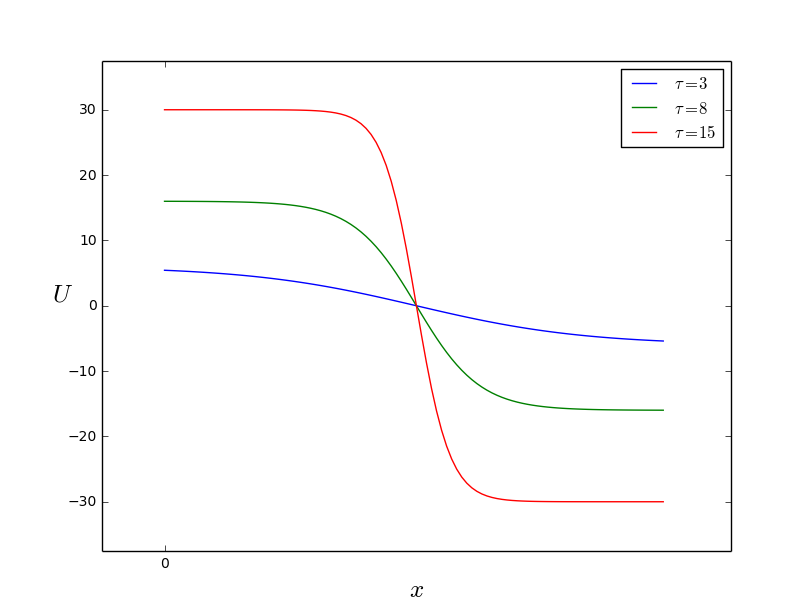
\includegraphics[width=4in]{fig1}
    \caption{$U(x)$ при разных $\sigma$}
\end{figure}

Для изучения устойчивости системы \eqref{fluct}, мы линеаризуем её

\begin{gather}\label{linearized}
    \theta_t = \theta_{xx} + 2 \sigma (\tanh(\sigma(x - \frac{1}{2}))\theta)_x \\*
    \theta(0, t) = \theta(1, t) = 0,
\end{gather}

где $\theta(x, t)$ - решение уравнения \eqref{linearized}, которое является
линеаризацией \eqref{fluct}. Заметим что \eqref{linearized} является  уравнение 
конвенкции-диффузии-реакции. Для простоты изучения устойчивости, мы избавимся 
от конвекционого члена используя преобразование 
$\zeta(x, t) = G(x)\theta(x, t)$, где 

\begin{equation}
    G(x) = \frac{\cosh(\sigma(x - \frac{1}{2}))}{\cosh(\frac{\sigma}{2})}
\end{equation} 

Имеем 

\begin{gather} \label{transf_linear}
    \zeta_t = \zeta_{xx} + \sigma^2 \left( \frac{2}{\cosh^2(\sigma(x - \frac{1}{2}))} - 1 \right) \zeta \\* 
    \zeta(0) = \zeta(1) = 0 
\end{gather}

Для $\sigma = 0$ система нейтрально устойчива. Для $\sigma > 0$, член 
$\left(\frac{2}{\cosh^2(\sigma(x - \frac{1}{2}))} - 1 \right)$  в 
\eqref{transf_linear} также является неустойчивым в окрестности 
$x = \frac{1}{2}$ (Рис 2.), т.е. положительность этого члена ведет к
неустойчивости системы


\begin{figure}[H]
    \centering
    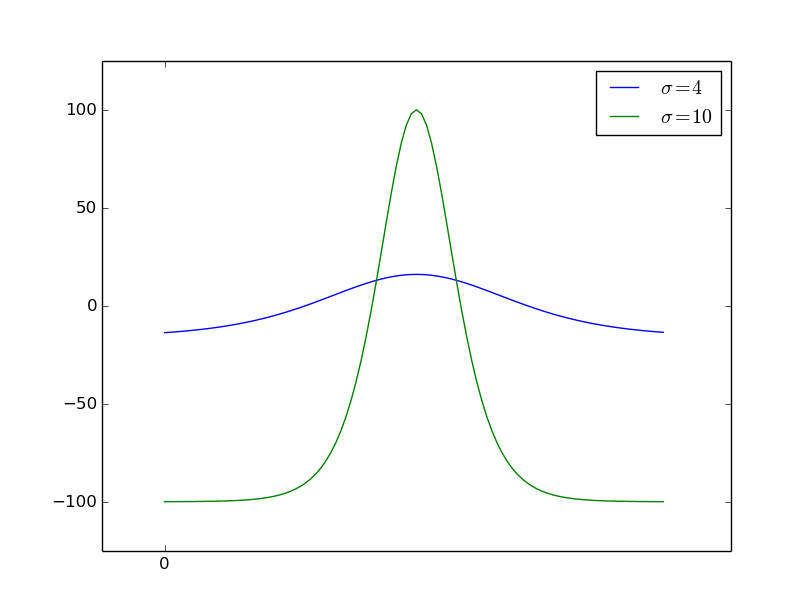
\includegraphics[width=4in]{fig2}
    \caption{Значение реакционного члена в \eqref{transf_linear}}
\end{figure}

    \section{Примеры неустойчивых стационарных решений}

Приведем численные примеры, демонстрирующие зависимость устойчивости
стационарного решения \eqref{shock_like} от параметра $\tau > 0$ и от
"возмущающих" гармоник $\theta_0$ (под гармоникой функции $\theta_0$ понимается
соответствующий компонент ряда Фурье в разложении $\theta_0$ по базису в $H$).
\newtheorem{exmp_bur}{Пример}
\begin{exmp_bur}
\end{exmp_bur}

Начальное условие $\theta_0(x) = \frac{\sin(\pi x)}{G(x)}$, параметр $\tau$ 
возмем равный 15. На рис. 7 показано неустойчивое поведение системы
\eqref{fluct}

\begin{figure}[h]
    \centering
    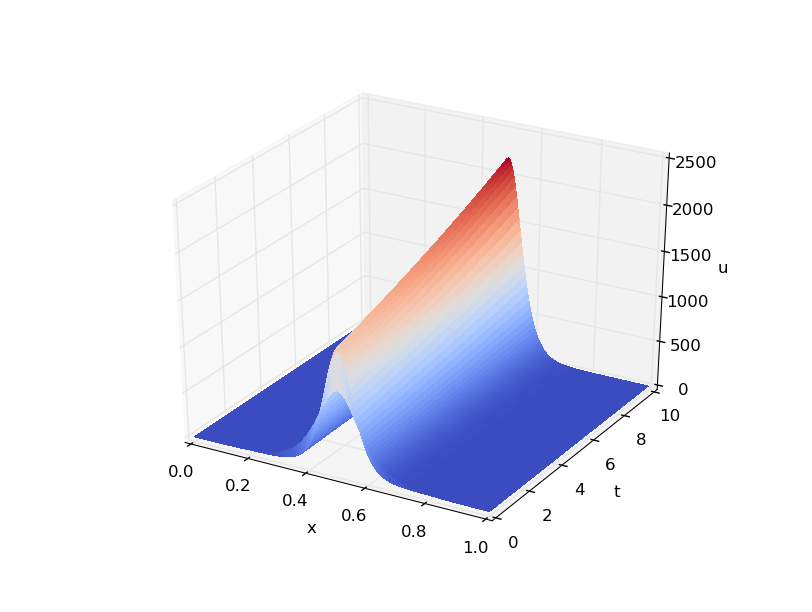
\includegraphics[width=3.0in]{ex_s15}
    \caption{}
    \label{fig:fig07}
\end{figure}

\begin{exmp_bur}
\end{exmp_bur}
Начальное условие $\theta_0(x) = \frac{x^2}{G(x)}$. Параметр $\tau = 15$.
Поведение решения представлено на рис.~\ref{fig:fig08}

\begin{figure}[h]
    \centering
    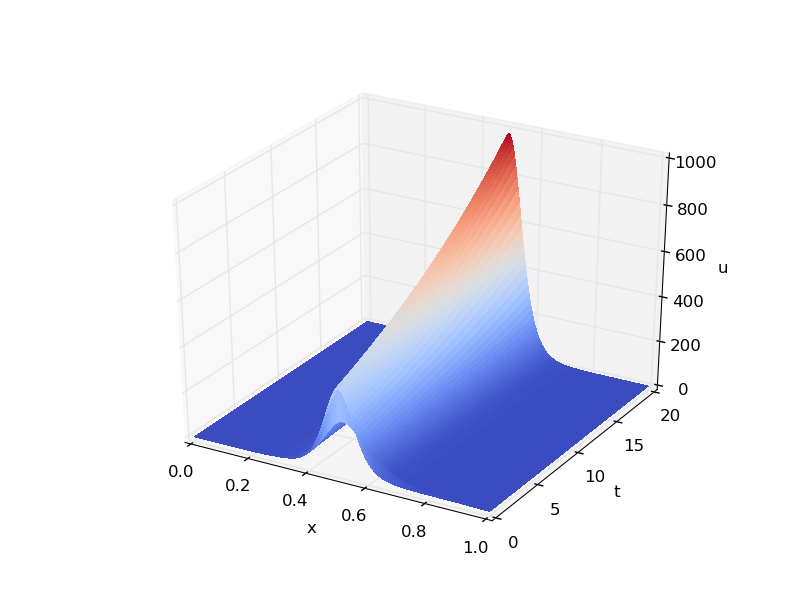
\includegraphics[width=3.0in]{ex_x2_s15}
    \caption{}
    \label{fig:fig08}
\end{figure}

    \section{Введение}

Пусть

\begin{equation}
    \Omega = (0, 1), \quad \omega \subset \Omega
\end{equation}

Неустойчивое уравнение Бюргерса

\begin{gather}
    y_t - \nu y_{xx} + yy_x = f \\*
    y|_{\partial \Omega} = y_{bi} \\*
    y|_{t=0} = y_0
\end{gather}

Стационарное уравнение Бюргерса

\begin{gather}
    y_{sxx} + y_s y_{sx} = f_s \\*
    y|_{s \partial \Omega} = y_{bi}
\end{gather}

\subsection{Задача стабилизации}
Найти оператор управления с обратной связью $\Lambda$ такой, что решение задачи
(1), где $f = f_s + \Lambda (y - y_s)$ экспоненциально сходится к $y_s$

Обозначим за $\varphi = y - y_s$, тогда

\begin{gather}
    \varphi_t - \nu \varphi_{xx} + y_s \varphi_x + \varphi y_{sx} + \varphi
    \varphi_x = \Lambda(\varphi) \\*
    \varphi_0 = y_0 - y_s \\*
    \varphi|_{\partial \Omega} = 0
\end{gather}

\subsection{Формализация}
Здесь и далее
\begin{equation}
    H = L^2(\Omega), \quad V = H^1_0(\Omega), \quad \norm{z}^2 = \int_{\Omega}{z^2dx}
\end{equation}

\begin{equation}
    V \subset H = H^{'} \subset V^{'} = H^{-1}(\Omega), (y, z) =
    \int_{\Omega}{yzdx}
\end{equation}

\begin{equation}
    A: V \rightarrow V^{'}, (Ay, z) = (y_x, z_x)
\end{equation}

\begin{equation}
    B: V \times V \rightarrow V^{'}, \quad (B(y, z), w) = (yz_x, w)
\end{equation}

\begin{equation}
    A w_j = \lambda_j w_j, \quad j = 1, 2.. \quad \lambda_j \rightarrow +\infty
\end{equation}

\begin{equation}
    \lambda_j = (\pi j)^2, \quad w_j(x) = \sqrt{2}\sin{(\pi j x)}
\end{equation}

Заметим что базис ортонормирован в $H$

\begin{equation}
    (w_j, w_k) = \delta_{jk}
\end{equation}

Введем следующие обозначения

\begin{equation}
    H_m = span{w_1, ..., w_m}, \quad P = P_m: H \rightarrow H_m, \quad Q=Q_m = I
    - P
\end{equation}

\subsubsection{Неравенства}

\begin{equation}
    \lambda_1 \norm{v}^2 \le \norm{v_x}^2, \quad \norm{v}^4_{L^4} \le \norm{v}^2
    \norm{v_x}^2
\end{equation}

\begin{equation}
    |(B(y, z), w)| \le \norm{y}_{L^4} \norm{z_x} \norm{w}_{L^4} \le
    \norm{y}^{1/2} \norm{y_x}^{1/2} \norm{z_x} \norm{w}^{1/2} \norm{w_x}^{1/2}
\end{equation}

\begin{equation}
    \norm{w}^2 \le \lambda^{-1}_{m + 1} \norm{w_x}^2 \forall w \in V \cap
    H_m^{\bot}
\end{equation}

\begin{equation}
    |v(x)| \le \norm{v_x}, \quad |(B(y, z), w)| \le \norm{y_x} \norm{z_x}
    \norm{w} \text{или} \norm{y} \norm{z_x} \norm{w_x}
\end{equation}

Оператор локально распределенного управления $\Lambda: H \rightarrow H$, \\
\begin{equation}
    \Lambda(\varphi) = -r \xi_{\omega}P\varphi
\end{equation}


Здесь \\
\begin{gather*}
    \begin{matrix}
        r & =
        & \left\{
        \begin{matrix}
            r_0, & 2 \norm{Q\varphi} \le \norm{P\varphi}, \quad r_0 > 0, \\
            0, & \mbox{иначе. }
        \end{matrix} \right.
    \end{matrix}, \quad
    \begin{matrix}
        \chi_{\omega}(x) & =
        & \left\{
        \begin{matrix}
            0, & \mbox{если } x \notin \omega, \\
            1, & \mbox{иначе. }
        \end{matrix} \right.
    \end{matrix}
\end{gather*}

Перепишем задачу в следующем виде

\begin{gather}
    \varphi' + \nu A\varphi + B(\varphi, y_s) + B(y_s + \varphi, \varphi) =
    \Gamma(\varphi), \quad t > 0 \\*
    \varphi(0) = \varphi_0 = y_0 - y_s
\end{gather}

\subsection{Разрешимость задачи на конечном интервале времени}

\newtheorem{theorem}{Теорема}

\begin{theorem}
    Пусть $y_s \in H^1, \quad \varphi_0 \in H, \quad T > 0$. Тогда $\exists$ решение
    задачи $\varphi \in C([0, T], H) \cap L^2(0, T, V), \varphi' \in L^2(0, T, V')$
\end{theorem}

\begin{remark}
    Пусть $h(\lambda)$ единичная функция Хевисайда, \\
    \begin{gather*}
        \begin{matrix}
            h(\lambda) & =
            & \left\{
            \begin{matrix}
                1, & \lambda \ge 0 \\
                0, & \lambda < 0
            \end{matrix} \right.
        \end{matrix}
    \end{gather*}

    , тогда оператор управления примит следующий вид

    \begin{equation}
        \Lambda(\varphi) = -r_0 h(-2\norm{Q\varphi} +
        \norm{P\varphi})\chi_{\omega}P\varphi
    \end{equation}

\end{remark}


\begin{proof}
    Пусть $\Omega > 0$. Выберим параметры $\sigma$, $r_0$, $m$ такие, что
    $\norm{g(t)}$ ограничена на $[0, +\infty)$. Здесь $g(t) = \varphi(t)e^{\sigma t}$
    \begin{gather*}
        g' + \nu Ag - \sigma g + B(g, y_s) + B(y_s + ge^{-\sigma t}, g) = -r_0 +
        h(\norm{Pg} - 2 \norm{Qg}) + \chi_{\omega}Pg\\*
        g(0) = \varphi_0
    \end{gather*}
    Пусть $p = Pg$, $q = Qg$. Рассмотрим интервал $(t_0, t_1)$, где $\norm{p(t)}
    \le 2 \norm{q(t)}$:
    \begin{gather*}
        g' + \nu Ag - \sigma g + B(g, y_s) + B(y_s + ge^{-\sigma t}, g) = 0, \quad
        t_0 < t < t_1\\
        \frac{1}{2}\frac{d}{dt}\norm{g}^2 + \norm{g_x}^2 - \sigma \norm{g}^2 +
        \frac{1}{2}(y_{sx}, g^2) = 0
    \end{gather*}

    \begin{gather*}
        \norm{g}^2 = \norm{p}^2 + \norm{q}^2 < 5\norm{q}^2 < 5\lambda^{-1}_{m +
        1}\norm{q_x} \le 5 \lambda^{-1}_{m + 1}\norm{g_x}^2
    \end{gather*}

    Пусть 
    \begin{equation}
        C_1 = \sigma + \frac{1}{2}max|y_{sx}|, \quad 5C_1\lambda^{-1}_{m + 1} <
        \frac{\nu}{2}
    \end{equation}

    Тогда отсюда 
    \begin{equation}
        \frac{d}{dt}\norm{g}^2 + \nu \norm{g_x} < 0
    \end{equation}

    Тогда следует

    \begin{equation}
        \norm{g(t_1)} < \norm{g(t_0)}
    \end{equation}

    Далее 
    \begin{gather*}
        \frac{1}{2}\frac{d}{dt}\norm{q}^2 + \nu \norm{q_x}^2 - \sigma \norm{q}^2 +
        ((y_s g)_x, q) + \frac{1}{2}e^{-\sigma t}((g^2)_x, q) = 0\\
        \norm{g_x}^2 = \norm{p_x}^2 + \norm{q_x}^2 \le \lambda_{m} \norm{p}^2 +
        \norm{q_x}^2 \le 5\norm{q_x}^2\\
        |(y_s g)_x, q)| \le C_0 \norm{g} \norm{q_x} < 5 C_0 \lambda^{-1}_{m + 1}
        \norm{q_x}^2, \quad C_0 = max|y_s|\\
        |((g^2)_x, q)| = |(g^2, q_x)| \le \norm{g} \norm{g_x} \norm{q_x}
    \end{gather*}
    
    Пусть теперь $\norm{p(t)} \ge 2 \norm{q(t)}, \quad t \in (t_0, t_1)$\\
    \begin{gather*}
        g' + \nu Ag - \sigma g + (y_s g)_x + \frac{1}{2} e^{-\sigma t} (g^2)_x +
        r_0 \chi_{\omega} P = 0
    \end{gather*}

    Заметим что
    \begin{gather*}
        \gamma |(p, q)_{L^2(\omega)}| \le \norm{p} \norm{q} \le \frac{1}{2}
        \norm{p}^2 \text{следует, что} \\
        \norm{p}^2_{L^2(\omega)} + \gamma (p,
        q)_{L^2(\omega)} \ge \frac{\gamma}{2}\norm{p}^2
    \end{gather*}
    
    \begin{gather*}
        \frac{1}{2} \frac{d}{dt} [ \norm{p}^2 + \nu [ \norm{p_x}^2 - \sigma [
        \norm{p}^2 + \gamma \norm{q}^2] ]  + ( (y_s g)_x, p + \gamma q) + \gamma
    \norm{q} \\* + \gamma\norm{q_x}^2] + \frac{1}{2} e^{-\sigma t} ( (g^2)_x, p +
    \sigma q) + \frac{r_0 \gamma}{2} \norm{p}^2 \le 0\\
    |( (y_s g)_x, p)| \le C_0 \norm{p_x} \norm{g} \le \frac{3}{2} C_0 \norm{p}
    \norm{p_x} \le \frac{\nu}{2} \norm{p_x}^2 + \frac{1}{2\nu}(\frac{3}{2}C_0)^2
    \norm{p}^2
    \end{gather*}

    \begin{equation}
        \norm{g} \le \norm{p} + \norm{q} \le \frac{3}{2} \norm{p}
    \end{equation}

    \begin{gather*}
        |((y_s g)_x, q)| \le C_0 \norm{q_x} \norm{g} \le \frac{3}{2} C_0
        \norm{q_x} \norm{p} \le \frac{\nu}{2} \norm{q_x}^2 + \frac{9C_0^2}{8\nu}
        \norm{p}^2
    \end{gather*}

    \begin{align*}
        \frac{d}{dt}(\norm{p}^2 + \gamma \norm{g}^2) + \nu(\norm{p_x}^2 + \gamma
        \norm{q_x}^2) + (r_0\gamma - (2 + \gamma)\sigma - (1 +
        \gamma)\frac{9C_0^2}{4\nu})\norm{p}^2 \\* \le |(g^2, p_x + \gamma q_x)|
    \end{align*}

    \begin{equation}
        r_0 > C_2 = (1 + \frac{2}{\gamma})\sigma + (1 +
        \frac{1}{\gamma})\frac{9C_0^2}{4\nu}
    \end{equation}

    Оценим правую часть 

    \begin{gather*}
        |(g^2, p_x + \gamma q_x)| = (1 - \gamma)|(g^2, p_x)| = (1 - \gamma)|(p^2
        + 2pq + q^2, p_x)| \\*
        = (1 - \gamma)|(q^2, p_x) - (p^2, q_x)| \le \norm{p_x} \norm{q_x}
        (\norm{p} + \norm{q}) \\* \le
        \frac{1}{2\sqrt{\gamma}}(\norm{p_x}^2 + \gamma \norm{q_x}^2)
        \frac{2}{\sqrt{\gamma}}\sqrt{\norm{p}^2 + \gamma \norm{q}^2}
    \end{gather*}
    т.к. $\norm{p} + \norm{q} \le \frac{2}{\sqrt{\gamma}}\sqrt{\norm{p}^2 +
        \gamma \norm{q}^2}$ отсюда следует, что

    \begin{equation}
        \frac{d}{dt}(\norm{p}^2 + \gamma \gamma{q}^2) + (\norm{p_x}^2 + \gamma
        \norm{q_x}^2) (\nu - \frac{1}{\nu} \sqrt{\norm{p}^2 + \gamma \norm{q}^2}
        \le 0
    \end{equation}

    
\end{proof}

    \subsection{Численная реализация алгоритма}
\vspace{1em}

В настоящем параграфе приведена численная реализация предложенного алгоритма 
стабилизации.\\

Рассмотрим задачу с стабилизирующим оператором

\begin{equation}\label{sys}
    u_t - u_{xx} - \alpha u = -r\chi_{\omega}P_m u, \ 0 < x < 1, \quad t > 0
\end{equation}

К уравнению \eqref{sys} добавим начальное и граничные условия

\begin{gather}\label{s_control}
    u(0, t) = u(1, t) = 0, \\*
    u(x, 0) = u_{0}(x) \in H. \nonumber
\end{gather}

Для \eqref{sys} запишем разностную схему

\begin{equation}\label{scheme}
    \frac{u^{j + 1}_i - u^j_i}{\tau} - \frac{u_{i + 1}^{j + 1} - 
    2u_{i}^{j + 1} + u_{i - 1}^{j + 1}}{h^2} - \alpha u_{i}^{j + 1} + 
    r\chi_{\omega}P_m u^j_i = 0.
\end{equation}

Запишем аппроксимацию начального и граничных условий

\begin{gather}
    u_i^0 = u_0(x_i), \\*
    u_1^{j+1} = u_N^{j+1} = 0. \nonumber
\end{gather}

Вспомним, что оператор проектирования имеет вид

\begin{gather*}
    P_m u = \sum \limits_{j=1}^{m} {(u, w_j) w_j} = 
    \sqrt{2} (\sum \limits_{j=1}^{m} {C_k \sin{(\pi k x)}}), \ \text{где }
    C_k = \sqrt{2} \int\limits_0^1{u(s)\sin{(\pi k s)} ds}.
\end{gather*}

Заметим, что $C_k$ - это интеграл от быстро осциллирующей функции вида

\begin{equation}
    \int\limits_a^b{f(x) e^{i\omega x} dx} \approx \int\limits_a^b{L_3(x)
    e^{i\omega x} dx}.
\end{equation}

Поскольку, функция $f$ является гладкой, то на $[a, b]$ она легко приближается 
с известной погрешностью интерполяционными многочленами. Пусть для 
определенности, это интерполяционный многочлен в форме Лагранжа

\begin{equation}
    L_3(x) = P_1(x)f(x_1) + P_2(x)f(x_2) + P_3(x)f(x_3)
\end{equation}
построенный по узлам $x_1 = a$, $x_2 = \frac{a + b}{2}$, $x_3 = b$. $P_i$ - 
многочлены второй степени, не зависящие от функции $f$. Данный метод 
приближенного интегрирования называется формулой Филона. Именно этим 
способом и будем аппроксимировать оператор $P_m$.\\

Для решения данной схемы \eqref{scheme} воспользуемся методом прогонки.

    \subsection{Примеры численного моделирования стабилизации неустойчивых решений}
\vspace{1em}

\subsubsection{Стабилизация неустойчивых решений}

\newtheorem{exmp_stbur}{Пример}

\begin{exmp_stbur}
\end{exmp_stbur}

Пусть $\theta_0 = \frac{sin(\pi x)}{G(x)}$ - начальное условие. Рассмотрим
стационарное решение уравнения Бюргерса с параметром $\tau$ возмем равный 15. 
В предыдущем параграфе показано неустойчивое поведение системы без управления. 
Cтабилизация указанного решения за счет управления с параметрами 
$\omega = (0, 0.4), \; r = 30, \; m = 4$ предоставлена ниже


\begin{figure}[H]
  \centering
  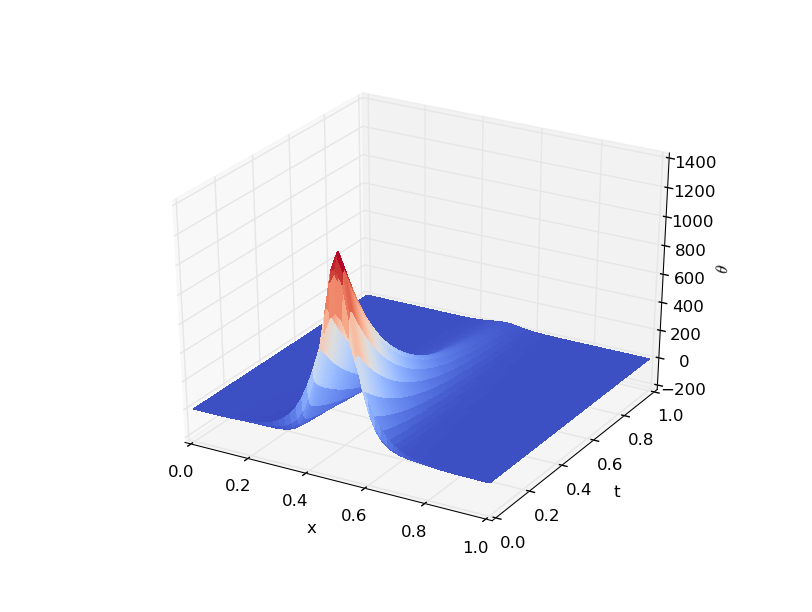
\includegraphics[width=3.5in]{re_s15}
  \caption{Управление с $\omega = (0, 0.4), \; m = 4, \; r = 30$}
  \label{fig:test2}
\end{figure}


\begin{exmp_stbur}
\end{exmp_stbur}
Пусть теперь начальное условие системы $\theta_0(x) = \frac{x^2}{G(x)}$.
Впспомним, что чем больше параметр $\tau > 0$, тем сильнее он влияет на
неустойчивость нашей системы \eqref{fluct}. Зафиксируем следующие параметры
стабилизирующего оператора управления $\omega = (0, 0.4), \ r = 30$, а параметр 
$\tau$  возмем равный $15$. Неустойчивость этой системы предемонстирована в
предыдущем параграфе (рис 2). Ниже представлен процесс стабилизации

\begin{figure}[H]
 \centering
  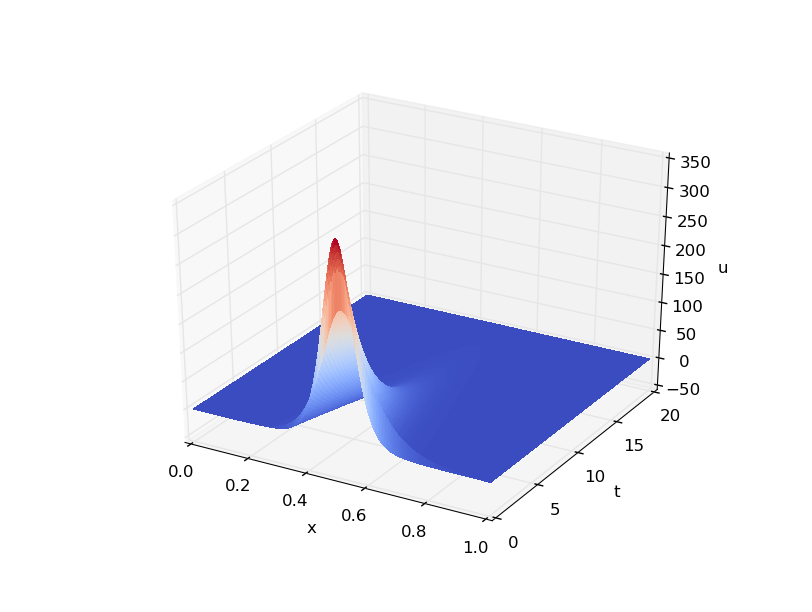
\includegraphics[width=4.0in]{re_x2_s15}
  \caption{$\omega = (0, 0.4), \; r = 30, \; m = 3$}
  \label{fig:test2}
\end{figure}

\subsubsection{Анализ параметров оператора стабилизации}
\vspace{1em}

В данном параграфе проанализируем зависимости параметров стабилизации.

\begin{exmp_stbur}
\end{exmp_stbur}

Рассмотрим неустойчивое решение системы \eqref{linearized}, где $\tau = 11$,
$\theta_0 = \frac{sin(5 \pi x)}{G(x)}$. Зафиксируем параметры стабилизирующего
оператора $\omega = (0, 0.3)$, $m = 2$. На графике представлена поведение решения
\eqref{linearized} от выбора параметра $r$.

\begin{figure}[H]
 \centering
  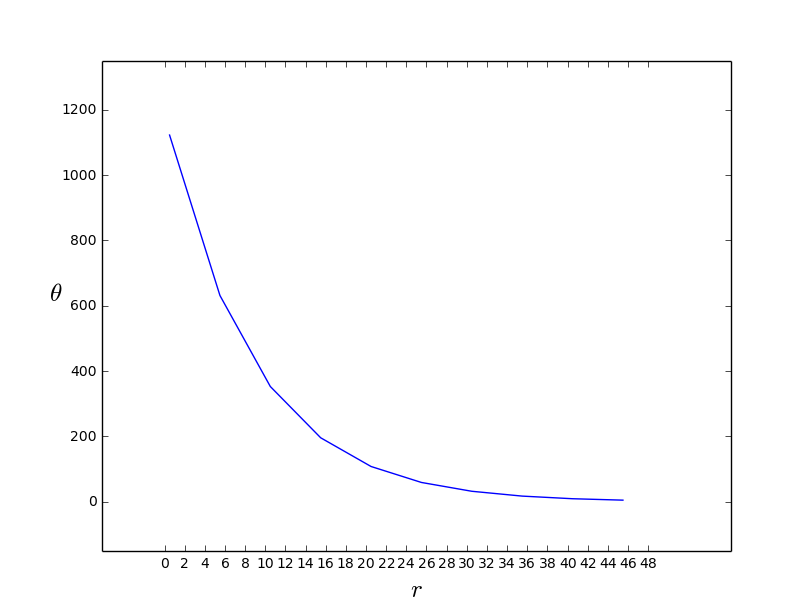
\includegraphics[width=4.5in]{r_m}
  \caption{$\omega = (0, 0.3), \; m = 2, \; r = 0.5, 5.5, ..., 45.5$}
  \label{fig:test2}
\end{figure}

\begin{exmp_stbur}
\end{exmp_stbur}

Начальное условие и параметр $\tau$ семейства стационарных решений типа
shock-like оставим теми же, что и в предыдущем примере. В этом примере мы
посмотрим поведение решение от выбора параметра $m$, при фиксированных $\omega =
(0, 0.3)$ и $r = 50$.

\begin{figure}[H]
 \centering
  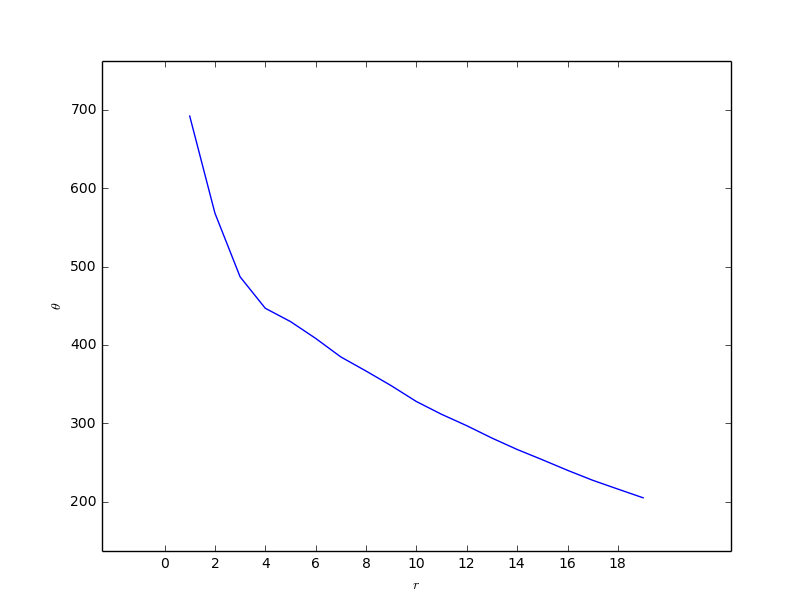
\includegraphics[width=4.5in]{m_r}
  \caption{$\omega = (0, 0.3), \; r = 50, \; m = 1, 2, .., 20$}
  \label{fig:test2}
\end{figure}

    %\section*{Заключение}
%\addcontentsline{toc}{section}{Заключение}
\Conclusion
\vspace{2em}

В представленной ВКР предложен простой метод стабилизации неустойчивых
стационарных решений параболических уравнений. Особенность предложенного
алгоритма заключается в локальности носителя управления и конечномерности образа
оператора управления. В работе получены следующие результаты:

\begin{itemize}

\item{Разработан алгоритм реализации стабилизирующего
управления для линейного уравнения теплопроводности и нелинейного уравнения
Бюргерса;}

\item{Проведён теоретический анализ устойчивости неустойчивых параболических
систем;}

\item{Реализован алгоритм стабилизации;}

\item{Приведены примеры неустойчивых стационарных решений, примеры численного 
моделирования стабилизации неустойчивых систем.}

\end{itemize}
%разработан алгоритм реализации стабилизирующего
%управления для линейного уравнения теплопроводности и нелинейного уравнения
%Бюргерса, теоретическое обоснование методов стабилизации, в том числе написание программы для решения разностных схем и
%реализация метода Филона для интегралов от быстро осциллирующих функций.
%Приведены примеры численного моделирования неустойчивых стационарных решений
%линейных параболических уравнений на примере уравнения теплопроводности и нелинейных для неустойчивых
%стационарных решений уравнения Бюргерса типа "shock-like", и применение
%предложенного алгоритма стабилизации.

    \section{Список литературы}
\vspace{2em}

\begingroup
\renewcommand{\section}[2]{}%
%\renewcommand{\chapter}[2]{}% for other classes
\begin{thebibliography}{}
\bibitem{}
	А.Ю. Чеботарёв, Конечномерная стабилизация с заданой скоростью систем типа Навье-Стокса. Дальневосточный мат. журнал 2010. Том 10 $№2$ с 200-205
\bibitem{oe04}
    M. Krstic, A. Smyshlyaev, Boundary Control of PDEs.\ 2008
\bibitem{}
	M. Krstic, A. Smyshlyaev, Boundary Control of PDEs (short course).\ 2006
\bibitem{}
    А. В. Фурсиков. Стабилизируемость квазилинейного параболического уравнения с помощью граничного управления с обратной связью. Матем. сб., 192:4 (.\ 2001)
\bibitem{}
	O.А. Ладыженская, Краевые задачи математической физики.\ 1973
\bibitem{}
	А.А. Самарский, А.В. Гулин, Численные методы. общий базовый курс.\ 1989
\bibitem{}
	Метод прогонки, неявная схема [Электронный ресурс] : \url{http://ikt.muctr.ru/html2/4/lek4_2_1.html}
\bibitem{}
	Формула Филона [Электронный ресурс] : \url{http://window.edu.ru/resource/886/19886/files/rsu177.pdf}

\end{thebibliography}
\endgroup
\end{onehalfspace}

\end{document} 
